\section{Resultados} \label{sec:results}

Esta seção discute os resultados da avaliação de desempenho proposta na Seção~\ref{sec:experiment}.
Os gráficos mostram a média das cinco execuções independentes,
com as barras de erro indicando o desvio padrão.
A análise foca em como a substituição do parâmetro $N$ pelo parâmetro $\rho$ impacta as métricas de avaliação.

\subsection{Cenário de Seleção Mínima ($\rho=0$ e $N=1$)}

As Figuras~\ref{fig:acc_1} e \ref{fig:loss_1} ilustram a acurácia e a perda de avaliação para o cenário de seleção mínima.
Nesta configuração, o FLASC é restringido a selecionar apenas o modelo com a menor perda local ($\rho=0$),
replicando exatamente a lógica de seleção rígida do FLSC com $N=1$.
Os resultados apontam que, em um regime de seleção unitária,
o uso do $\rho$ mantém desempenho similar ao da linha de base conforme teorisado na Seção~\ref{sec:experiment}.

\begin{figure}[H]
    \centering
    \begin{minipage}{0.48\textwidth}
        \centering
        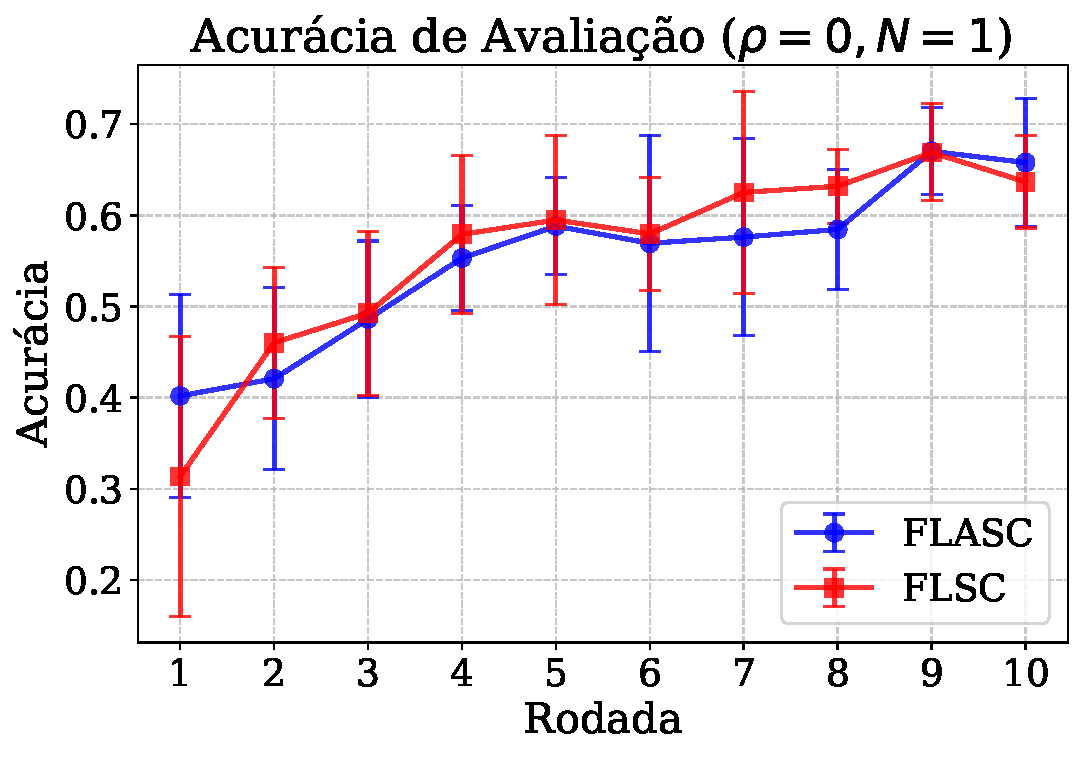
\includegraphics[width=\textwidth]{figs/eval_accuracy_1.pdf}
        \caption{Evolução da acurácia de avaliação no cenário de seleção mínima ($\rho=0, N=1$).}
        \label{fig:acc_1}
    \end{minipage}
    \hfill
    \begin{minipage}{0.48\textwidth}
        \centering
        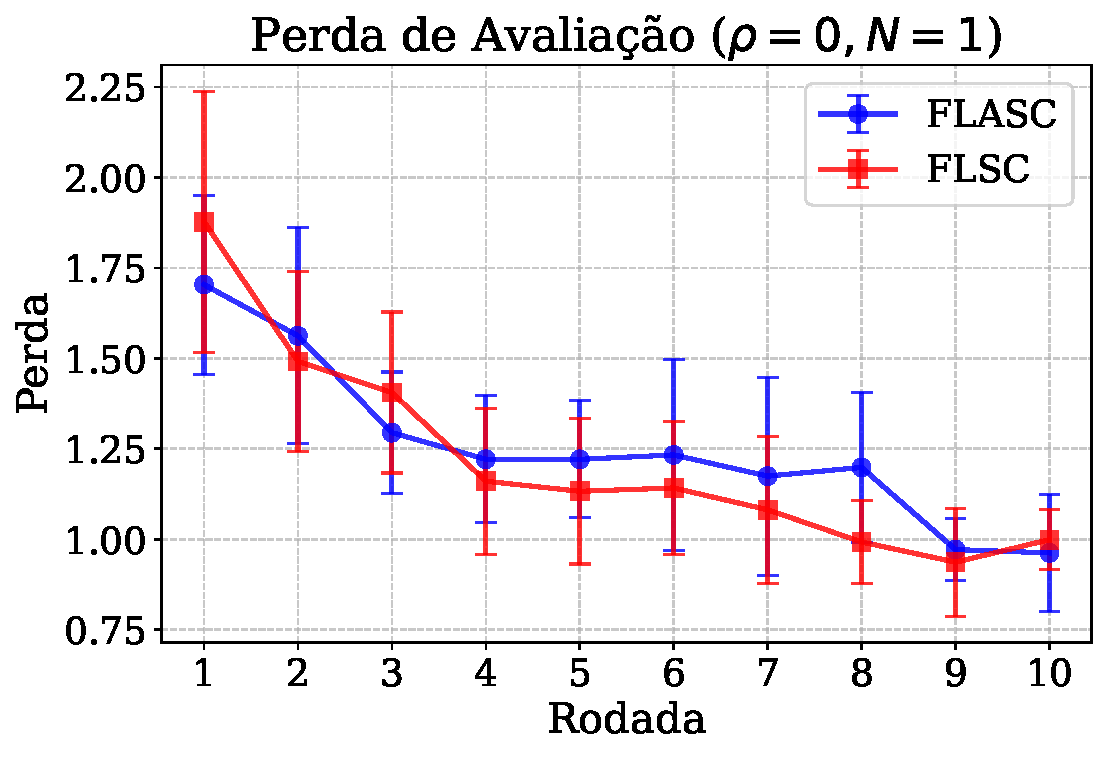
\includegraphics[width=\textwidth]{figs/eval_loss_1.pdf}
        \caption{Evolução da perda de avaliação no cenário de seleção mínima ($\rho=0, N=1$).}
        \label{fig:loss_1}
    \end{minipage}
\end{figure}

\subsection{Cenário de Seleção Intermediária ($\rho=0,5$ e $N=2$)}

No cenário intermediário, as Figuras~\ref{fig:acc_2} e \ref{fig:loss_2} mostram que o FLASC e o FLSC mantiveram comportamentos similares.
Havia a expectativa de que o limiar adaptativo $\rho$ permitisse um refinamento na seleção, 
filtrando modelos com desempenho marginal e favorecendo a estabilidade. 
Entretanto, a imposição de um número fixo de modelos ($N=2$) no FLSC não se mostrou prejudicial.

\begin{figure}[H]
    \centering
    \begin{minipage}{0.48\textwidth}
        \centering
        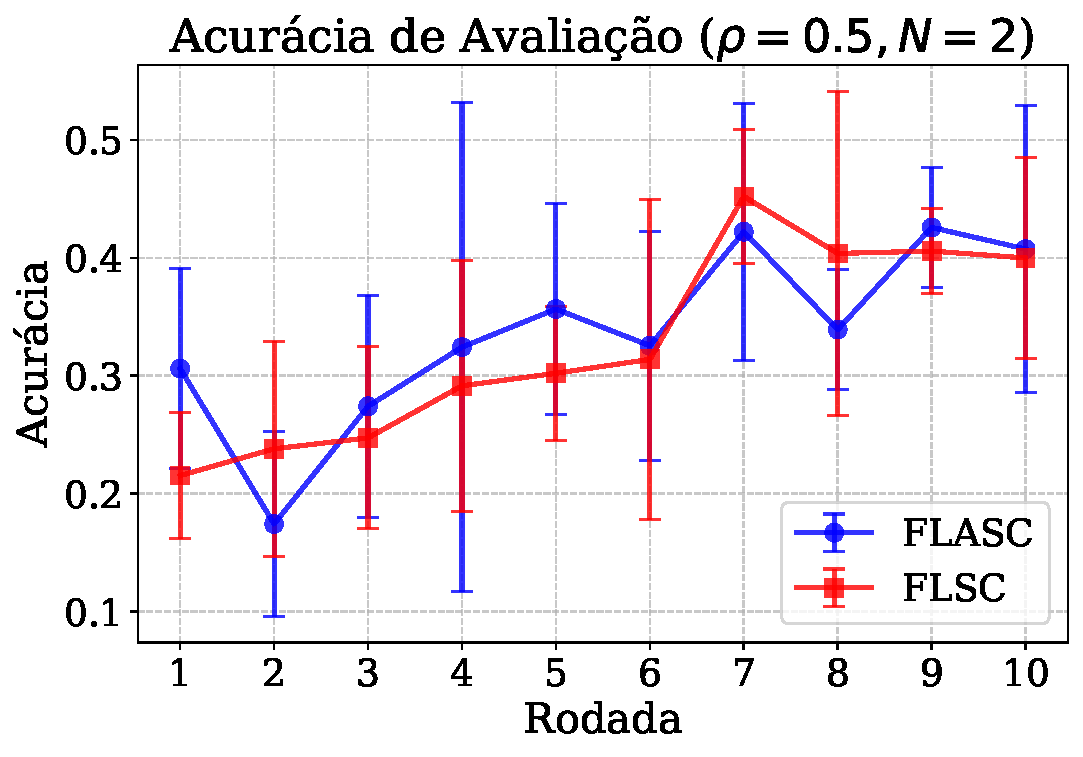
\includegraphics[width=\textwidth]{figs/eval_accuracy_2.pdf}
        \caption{Evolução da acurácia de avaliação no cenário intermediário ($\rho=0,5, N=2$).}
        \label{fig:acc_2}
    \end{minipage}
    \hfill
    \begin{minipage}{0.48\textwidth}
        \centering
        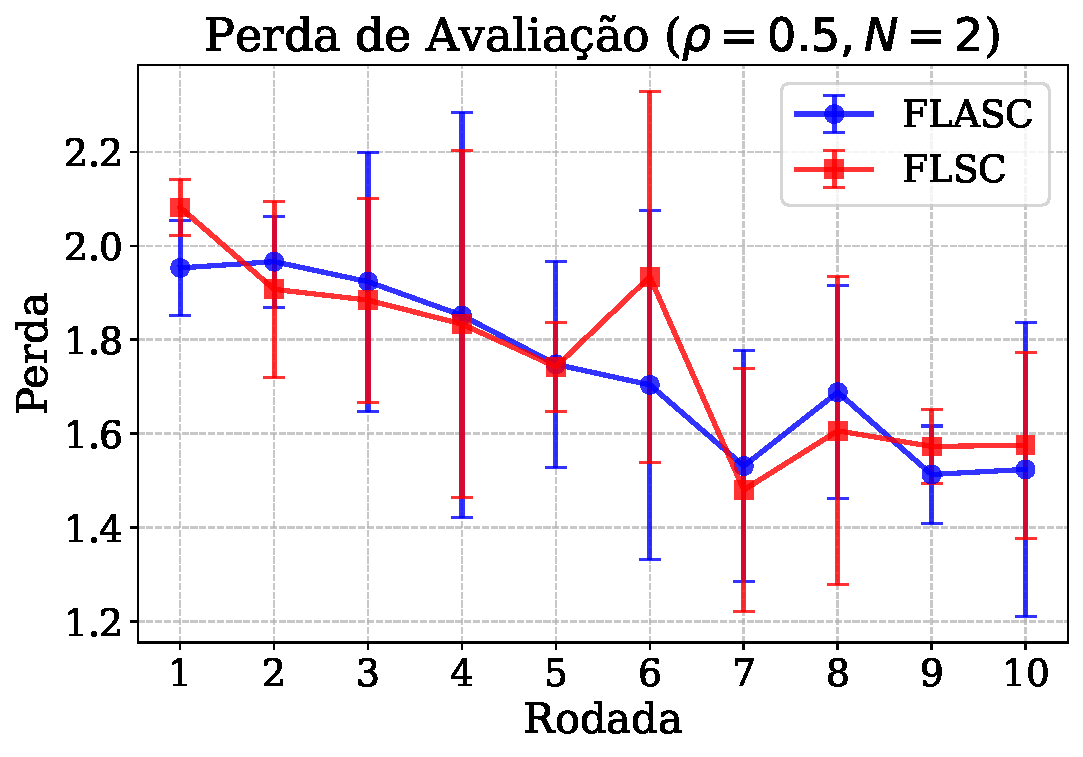
\includegraphics[width=\textwidth]{figs/eval_loss_2.pdf}
        \caption{Evolução da perda de avaliação no cenário intermediário ($\rho=0,5, N=2$).}
        \label{fig:loss_2}
    \end{minipage}
\end{figure}

\subsection{Cenário de Seleção Máxima ($\rho=1$ e $N=4$)}

Para o cenário de seleção máxima, as Figuras~\ref{fig:acc_3} e \ref{fig:loss_3}
revelam que a ponderação das perdas na fusão local não proporcionou ganhos significativos ao FLASC.
Embora a hipótese central fosse de que priorizar modelos com melhor adaptação local resultaria em uma convergência acelerada, 
os dados indicam que tanto a média ponderada quanto a média simples (FLSC) convergem para patamares de acurácia equivalentes.

\begin{figure}[H]
    \centering
    \begin{minipage}{0.48\textwidth}
        \centering
        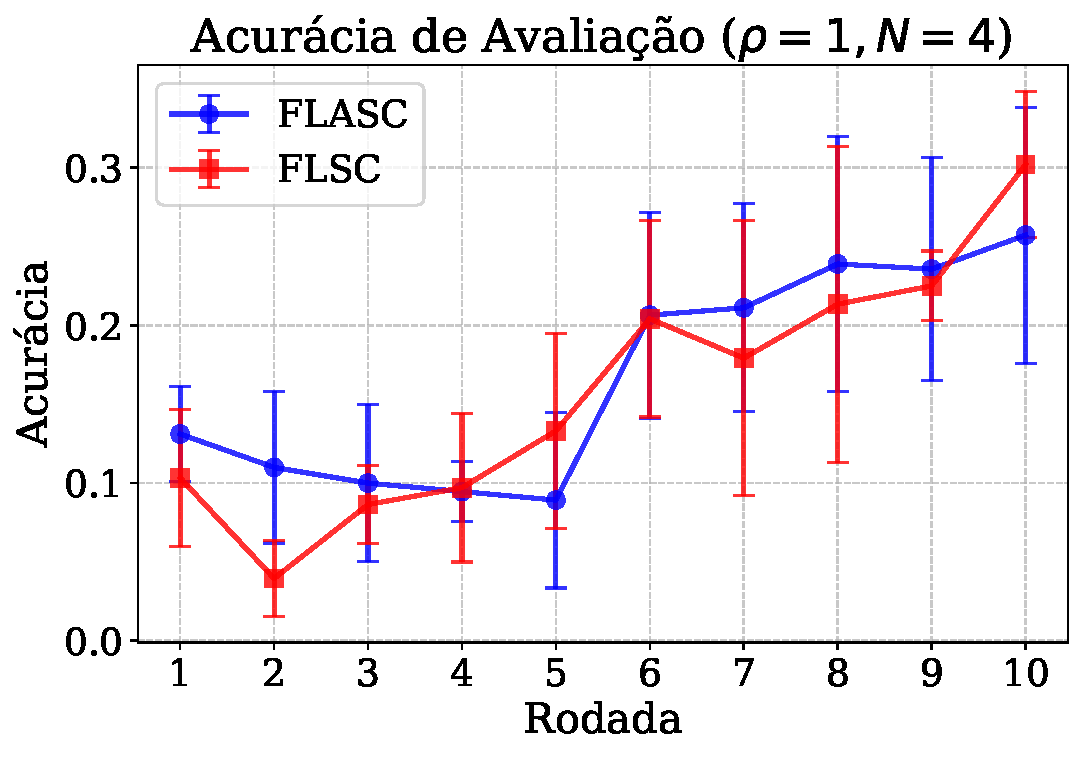
\includegraphics[width=\textwidth]{figs/eval_accuracy_3.pdf}
        \caption{Evolução da acurácia de avaliação no cenário de seleção máxima ($\rho=1, N=4$).}
        \label{fig:acc_3}
    \end{minipage}
    \hfill
    \begin{minipage}{0.48\textwidth}
        \centering
        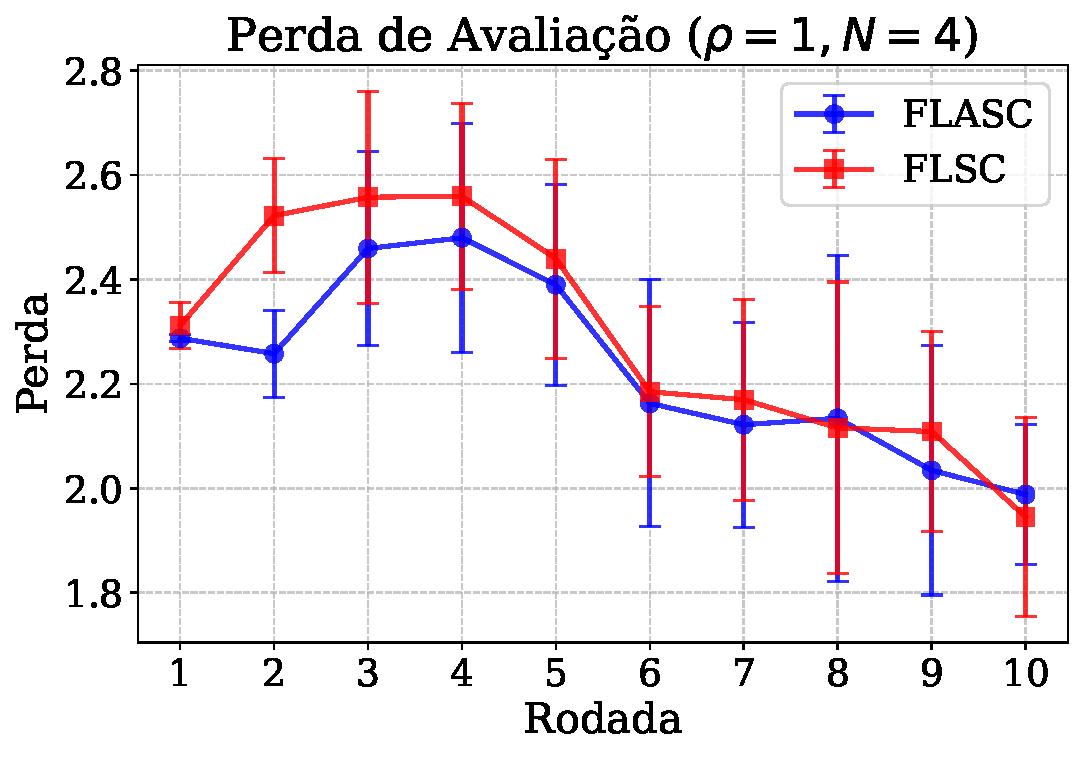
\includegraphics[width=\textwidth]{figs/eval_loss_3.pdf}
        \caption{Evolução da perda de avaliação no cenário de seleção máxima ($\rho=1, N=4$).}
        \label{fig:loss_3}
    \end{minipage}
\end{figure}

Em suma, os resultados mostram que a troca de parâmetros rígidos pelo 
mecanismo adaptativo proposto, embora ofereça maior flexibilidade teórica,
não resultou em diferença expressiva de desempenho no cenário experimental avaliado.
